\begin{frame}{}
    \LARGE NLP: \textbf{Basics}
\end{frame}

\begin{frame}{What is NLP?}
    \begin{itemize}
        \item NLP stands for Natural Language Processing.
        \item It helps computers understand and work with human languages, like English or Arabic.
        \item With NLP, computers can read, listen, write, or even talk like humans.
        \item Examples: chatbots, language translators, voice assistants.
    \end{itemize}
\end{frame}

\begin{frame}[allowframebreaks]{Text Data is Superficial}
An iceberg is a large piece of freshwater ice that has broken off
from a snow-formed glacier or ice shelf and is floating in open
water.
\begin{figure}
    \centering
    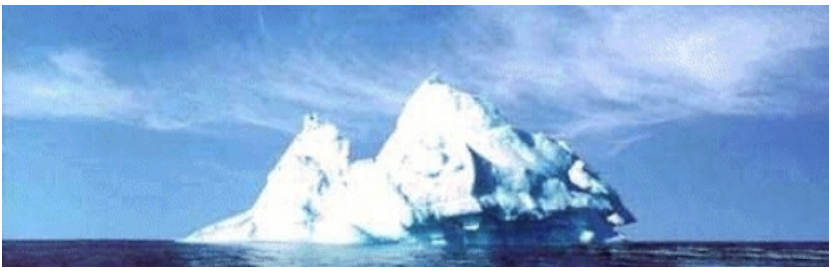
\includegraphics[height=0.9\textheight, width=\textwidth, keepaspectratio]{images/nlp/intro_slide_4_1_img.png}
\end{figure}

\end{frame}

\begin{frame}[allowframebreaks]{.. But Language is Complex}
\begin{columns}
    \begin{column}{0.55\textwidth}
        \begin{figure}
            \centering
            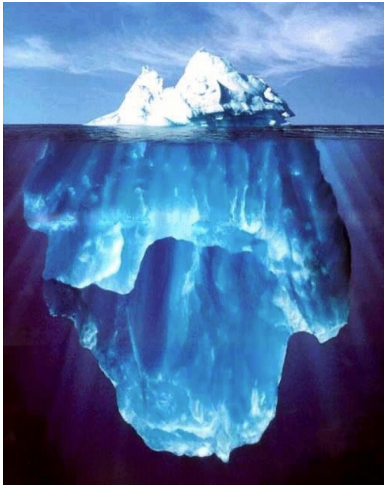
\includegraphics[height=0.9\textheight, width=\textwidth, keepaspectratio]{images/nlp/intro_slide_5_1_img.png}
        \end{figure}
    \end{column}
    \begin{column}{0.45\textwidth}
        An iceberg is a large piece of freshwater ice that has broken off
        from a snow-formed glacier or ice shelf and is floating in open
        water.
    \end{column}
\end{columns}
\end{frame}

\begin{frame}[allowframebreaks]{NLP Basics – What It’s All About}
Teaching machines to \textbf{understand and generate human language}
\vspace{-1em}
\begin{itemize}
    \item \textbf{Text preprocessing}: \\
    {\small Cleaning and preparing raw text data (removing noise, tokenization, normalization).}
    \item \textbf{Understanding meaning}: \\
    {\small Extracting meaning from text using techniques like part-of-speech tagging, named entity recognition, and sentiment analysis.}
    \item \textbf{Language modeling}: \\
    {\small Building models that can predict or generate text, such as autocomplete or next-word prediction.}
    \item \textbf{Translation, summarization, etc.}: \\
    {\small Enabling applications like machine translation, text summarization, question answering, and more.}
\end{itemize}

\textcolor{blue}{Text data is everywhere: tweets, reviews, articles, chats! NLP helps us make sense of this vast information.}

\end{frame}

\begin{frame}[allowframebreaks]{Core NLP Tasks}
\begin{table}[ht]
    \centering
    \renewcommand{\arraystretch}{1.8} % Increased row spacing
    \begin{tabular}{@{} p{0.3\textwidth} p{0.3\textwidth} p{0.4\textwidth} @{}}
        \toprule
        \textbf{Task} & \textbf{What It Does} & \textbf{Example} \\
        \midrule
        \hline % Horizontal line after header row
        \textbf{Tokenization} & Split text into words & \texttt{"I love NLP"} $\rightarrow$ \texttt{["I", "love", "NLP"]} \\
        \textbf{POS Tagging} & Label grammar tags & \texttt{"Dogs bark"} $\rightarrow$ [Noun, Verb] \\
        \textbf{Named Entity Recognition} & Find names, places, etc. & \texttt{"Christopher Nolan lives in Los Angeles"} \\
        \textbf{Sentiment Analysis} & Detect mood & \texttt{"This movie was amazing!"} $\rightarrow$ Positive \\
        \textbf{Machine Translation} & Language to language & English $\rightarrow$ French \\
        \bottomrule
    \end{tabular}
    \caption*{Core NLP Tasks and Examples}
\end{table}
\end{frame}


\begin{frame}{Text Preprocessing}
    \begin{itemize}
        \item \textbf{Lowercase everything}: \\
        {\small Example: \texttt{"NLP"} $\rightarrow$ \texttt{"nlp"}}
        \item \textbf{Removing stop words}: \\
        {\small Eliminate common words that carry little meaning (e.g., "is", "the", "and") to focus on important content.}
        \item \textbf{Stemming/Lemmatization}: \\
        {\small Reduce words to their root or base form. \\
        Example: \texttt{"running"} $\rightarrow$ \texttt{"run"}}
        \item \textbf{Vectorization}: \\
        {\small Transform words or documents into numerical representations for machine learning models:
        \begin{itemize}
            \item \textbf{Bag of Words}: Counts word occurrences in a document.
            \item \textbf{TF-IDF (Term Frequency-Inverse Document Frequency)}: Weighs words by importance across documents.
            \item \textbf{Word2Vec}: Learns dense vector representations capturing word meaning and context.
        \end{itemize}}
    \end{itemize}
\end{frame}

\begin{frame}{What is Vocabulary in NLP?}
    \begin{itemize}
        \item \textbf{Vocabulary} = All unique words in your dataset
        \item Example: \texttt{"I love NLP and NLP loves me"} $\rightarrow$ \\
        Vocabulary = \{\texttt{"I"}, \texttt{"love"}, \texttt{"NLP"}, \texttt{"and"}, \texttt{"loves"}, \texttt{"me"}\}
        \item More data = Bigger vocabulary = Harder to process!
    \end{itemize}
    \vspace{1em}
    \textcolor{blue}{\faLightbulbO\enspace Tip: Rare words may not help; common words may not mean much.}
\end{frame}

\begin{frame}{The Problem with Sparse Representations}
    \textbf{Traditional approach: One-hot encoding}
    \begin{itemize}
        \item Example: \texttt{"NLP"} $\rightarrow$ [0, 0, 1, 0, 0, 0, 0\ldots]
    \end{itemize}
    \vspace{1em}
    \textbf{Problem:}
    \begin{itemize}
        \item High-dimensional (thousands of words!)
        \item Sparse (mostly 0s)
        \item No meaning in structure (no relation between \texttt{"king"} and \texttt{"queen"})
        \item \textcolor{red}{\faTimes\enspace Not efficient for learning}
    \end{itemize}
\end{frame}

\begin{frame}{Word Frequencies \& Feature Extraction}
    \textbf{Feature extraction = Turning text into numbers}
    \begin{itemize}
        \item Count how often each word appears (\textbf{Term Frequency})
    \end{itemize}
    \vspace{1em}
    \textbf{Example:}
    \begin{table}[ht]
        \centering
        \renewcommand{\arraystretch}{1.8} % Increased row spacing
        \begin{tabular}{lcc}
            \toprule
            \textbf{Text} & \texttt{"great product"} & \texttt{"bad product"} \\
            \midrule
            Word: \texttt{"great"} & 1 & 0 \\
            Word: \texttt{"bad"} & 0 & 1 \\
            \bottomrule
        \end{tabular}
    \end{table}
    \vspace{0.5em}
    \textcolor{blue}{\faBalanceScale\enspace Use this to find patterns in sentiment, spam, etc.}
\end{frame}

\begin{frame}{Positive \& Negative Frequencies}
    Suppose you're classifying reviews:

    \vspace{0.5em}
    \textbf{Positive Reviews:} \texttt{["amazing", "good", "great"]} \\
    \textbf{Negative Reviews:} \texttt{["bad", "awful", "terrible"]}

    \vspace{1em}
    Count how often each word appears in each class.

    \vspace{1em}
    \textbf{Example table:}
    \begin{table}[ht]
        \centering
        \renewcommand{\arraystretch}{1.5}
        \begin{tabular}{lcc}
            \toprule
            \textbf{Word} & \textbf{Positive Count} & \textbf{Negative Count} \\
            \midrule
            good & 20 & 1 \\
            bad & 1 & 30 \\
            \bottomrule
        \end{tabular}
    \end{table}

    \vspace{0.5em}
    Helps models detect the “tone” (\textbf{sentiment clues}) of new text.
\end{frame}

\begin{frame}{Feature Extraction Techniques}
    \begin{itemize}
        \item \textbf{Bag of Words (BoW)}: Just counts word frequencies in each document.
        \item \textbf{TF-IDF (Term Frequency-Inverse Document Frequency)}: Adjusts for how “unique” or important a word is in a document compared to all documents.
        \begin{itemize}
            \item Words like \texttt{"the"}, \texttt{"is"} are less important.
        \end{itemize}
        \item \textbf{Word Embeddings (later)}: Add meaning and capture relationships between words (e.g., similarity, analogy).
    \end{itemize}
\end{frame}

\begin{frame}{N-Gram Models – Capture Word Pairs!}
    \textbf{BoW ignores word order:} \texttt{"not good"} = \texttt{"good"}

    \vspace{1em}
    \textbf{N-grams fix this:}
    \begin{itemize}
        \item \textbf{1-gram:} \texttt{"I"}, \texttt{"love"}, \texttt{"cats"}
        \item \textbf{2-gram:} \texttt{"I love"}, \texttt{"love cats"}
    \end{itemize}

    \vspace{1em}
    \textbf{Helps detect phrases:}
    \begin{itemize}
        \item \texttt{"not good"} $\neq$ \texttt{"very good"}
    \end{itemize}

    \vspace{1em}
    \textcolor{blue}{\faLightbulbO\enspace Bi-grams and tri-grams make models more context-aware!}
\end{frame}

\begin{frame}{Probabilities in NLP}
    NLP is all about uncertainty!

    \vspace{1em}
    We ask: \textbf{What is the probability that this sentence is positive?}

    \vspace{1em}
    \textbf{Example:}
    \begin{itemize}
        \item $P(\text{Positive} \mid \text{``great product''}) = 0.92$
        \item $P(\text{Negative} \mid \text{``great product''}) = 0.08$
    \end{itemize}
\end{frame}

\begin{frame}{Bayes’ Rule – A Quick Look}
    \textbf{Bayes’ Rule:}
    \[
        P(\text{Class} \mid \text{Words}) = \frac{P(\text{Words} \mid \text{Class}) \cdot P(\text{Class})}{P(\text{Words})}
    \]
    \vspace{1em}
    \begin{itemize}
        \item Predict class (e.g., spam or not) given the words
        \item Simple, powerful tool used in Naive Bayes classifiers
        \item Helps models reason with uncertainty
    \end{itemize}
\end{frame}

\begin{frame}{Naive Bayes for Sentiment Analysis}
    \textbf{Simple, fast probabilistic model}

    \vspace{1em}
    \textbf{Assumes:}
    \begin{itemize}
        \item Words are independent given the class (a “naive” assumption)
    \end{itemize}

    \vspace{1em}
    \textbf{Example:}
    \begin{itemize}
        \item \texttt{"This movie is awesome"} $\rightarrow$ $P(\text{Positive})$ high
        \item \texttt{"This movie is boring"} $\rightarrow$ $P(\text{Negative})$ high
    \end{itemize}

    \vspace{1em}
    \textcolor{green}{\faCheck\enspace Works well with BoW, TF-IDF, and N-grams}
\end{frame}

\begin{frame}[allowframebreaks]{Logistic Regression for Text Classification}
    We’re already familiar with probability-based classifiers, and have seen logistic regression applied in computer vision tasks.

    \vspace{1em}
    \begin{itemize}
        \item Here, logistic regression takes word features (from BoW or TF-IDF)
        \item It learns weights to predict if text belongs to a certain class, such as:
        \begin{itemize}
            \item Positive or Negative
            \item Spam or Not Spam
        \end{itemize}
        \item Outputs a probability:
        \[
            P(\text{Class} = 1 \mid \text{features}) = \sigma(w_1x_1 + w_2x_2 + \ldots + b)
        \]
        \item Words like “awesome” get high weights for positive class
    \end{itemize}

    \framebreak
    \textcolor{blue}{\faBullseye\enspace \textbf{Intuition:}}
    \begin{itemize}
        \item Each word contributes a “vote” toward a class.
        \item The model learns which words are most important for classification.
    \end{itemize}

    \framrbreak
    \begin{figure}
        \centering
        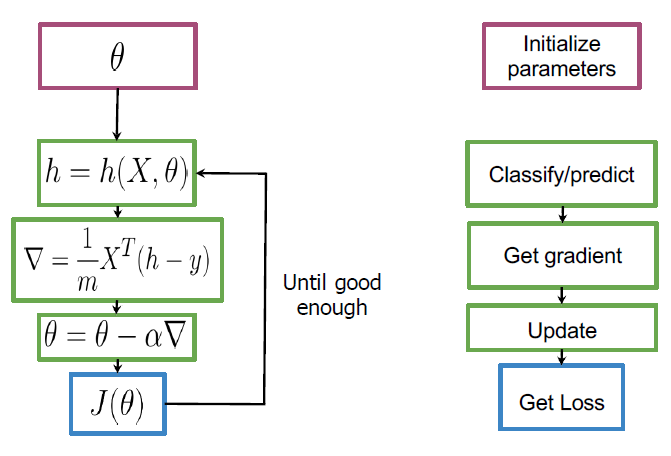
\includegraphics[height=0.85\textheight, width=\textwidth, keepaspectratio]{images/nlp/training-lr.png}
        \caption*{Training a Logistic Regression Model}
    \end{figure}
\end{frame}

\begin{frame}{Word Vectors – Adding Meaning!}
    \textbf{Unlike BoW, word vectors (embeddings) capture meaning}

    \vspace{1em}
    Words are mapped to dense vectors in low-dimensional space.

    \vspace{1em}
    \textbf{Example:} 300-dimensional vector: \texttt{"cat"} $\rightarrow$ [0.1, -0.3, ..., 0.2]

    \vspace{1em}
    \textbf{Similar words have similar vectors:}
    \begin{itemize}
        \item \texttt{"king"} and \texttt{"queen"} are close in vector space
        \item Captures relationships and analogies (e.g., \texttt{"man"} : \texttt{"woman"} :: \texttt{"king"} : \texttt{"queen"})
    \end{itemize}

    \vspace{1em}
    \textcolor{blue}{\faLightbulbO\enspace Word embeddings add context and meaning to NLP models!}
\end{frame}

\begin{frame}{Popular Word Vector Models}
    \begin{itemize}
        \item \textbf{Word2Vec (Google):} \\
        Trains using context words (“You shall know a word by the company it keeps”)
        \item \textbf{GloVe (Stanford):} \\
        Uses word co-occurrence in large corpus
        \item \textbf{FastText (Facebook):} \\
        Captures subword info, works better for rare words
    \end{itemize}
    \vspace{1em}
    \textcolor{green}{\faCheck\enspace Used for initializing deep models like RNNs, Transformers}
\end{frame}

\begin{frame}{Recap – NLP Basics}
    \begin{itemize}
        \item \textbf{Vocabulary and word counts} are key features for representing text.
        \item \textbf{Sparse data} (like one-hot vectors) limits early NLP models.
        \item \textbf{Naive Bayes} and \textbf{Logistic Regression} are fast and effective for text classification.
        \item \textbf{N-grams} add word order and context.
        \item \textbf{Word vectors} (embeddings) bring semantic meaning to models.
    \end{itemize}
    \vspace{1em}
    Now, let’s dive into neural networks for language...
\end{frame}